\documentclass[11pt,a4paper]{article}

% Allow embedding PDF 1.7 figures produced by GraphViz.
\pdfminorversion=7

\usepackage[T1]{fontenc}
\usepackage{lmodern}
\usepackage{microtype}
\usepackage{graphicx}
\usepackage{hyperref}
\usepackage{booktabs}
\usepackage{amsmath}
\usepackage{enumitem}
\usepackage{xcolor}
\usepackage{tikz}
\usetikzlibrary{calc,positioning,fit,shapes.geometric,arrows.meta,backgrounds,decorations.pathreplacing,decorations.pathmorphing}

\hypersetup{colorlinks=true, linkcolor=blue, urlcolor=blue, citecolor=blue}
\graphicspath{{diagrams/out/}}

\sloppy

% =============================================================================
% Draft watermark. Flip \draftmarkfalse below to disable for a final build.
% =============================================================================
\newif\ifdraftmark
\draftmarktrue
\ifdraftmark
  \usepackage{draftwatermark}
  \SetWatermarkText{\textsf{\bfseries DRAFT}}
  \SetWatermarkScale{1.10}
  \SetWatermarkLightness{0.97}
\fi

% =============================================================================
% Shared TikZ vocabulary used by Figures 1 and 2.
% Color choices match the existing GraphViz figures so the paper reads as a
% consistent visual system: orange = unguided/LLM-managed, green = guided/
% procedure-owned, blue = task/protocol substrate.
% =============================================================================
\definecolor{ungOrange}{HTML}{D17A4A}
\definecolor{ungBg}{HTML}{FFF2EC}
\definecolor{guGreen}{HTML}{3F8A4A}
\definecolor{guBg}{HTML}{ECF6EE}
\definecolor{taskBlue}{HTML}{3B6FB6}
\definecolor{taskBg}{HTML}{EAF1FB}
\definecolor{oobAmber}{HTML}{B89B3A}
\definecolor{oobBg}{HTML}{FFFCEE}
\definecolor{rulegray}{HTML}{888888}

\tikzset{
    actor/.style={draw=rulegray, fill=white, rounded corners=2pt,
                  font=\sffamily\small\bfseries, inner sep=4pt, minimum width=22mm,
                  align=center},
    lifeline/.style={draw=rulegray, dashed, line cap=round},
    msg/.style={-{Stealth[length=2.2mm]}, line width=0.45pt, font=\sffamily\scriptsize},
    msglbl/.style={font=\sffamily\scriptsize, fill=white, inner sep=1pt, align=center},
    selfmsg/.style={-{Stealth[length=2mm]}, line width=0.45pt, font=\sffamily\scriptsize},
    note/.style={draw=oobAmber, fill=oobBg, rounded corners=2pt, dashed,
                 font=\sffamily\scriptsize\itshape, inner sep=4pt, align=center,
                 line width=0.5pt},
    panelTitleU/.style={font=\sffamily\bfseries, color=ungOrange},
    panelTitleG/.style={font=\sffamily\bfseries, color=guGreen},
    sysCard/.style={draw=taskBlue, fill=taskBg, rounded corners=2pt,
                    font=\ttfamily\scriptsize, inner sep=4pt, align=left,
                    text width=58mm, line width=0.6pt},
    sysCardSmall/.style={draw=taskBlue, fill=taskBg, rounded corners=2pt,
                         font=\ttfamily\scriptsize, inner sep=4pt, align=left,
                         text width=58mm, line width=0.6pt},
    userCard/.style={draw=ungOrange!70, fill=ungBg, rounded corners=2pt,
                     font=\ttfamily\scriptsize, inner sep=4pt, align=left,
                     text width=58mm, line width=0.5pt},
    userCardG/.style={draw=guGreen!70, fill=guBg, rounded corners=2pt,
                      font=\ttfamily\scriptsize, inner sep=4pt, align=left,
                      text width=58mm, line width=0.5pt},
    asstCard/.style={draw=rulegray, fill=white, rounded corners=2pt,
                     font=\ttfamily\scriptsize, inner sep=4pt, align=left,
                     text width=58mm, line width=0.5pt},
    roleTag/.style={font=\sffamily\scriptsize\bfseries, inner sep=1pt},
    oobCallout/.style={draw=oobAmber, fill=oobBg, rounded corners=3pt, dashed,
                       inner sep=5pt, align=left, font=\ttfamily\scriptsize,
                       text width=58mm, line width=0.6pt},
}

\title{Procedure-Owned Elicitation Checkpoints vs.\ LLM-Managed Capture\\
A Controlled Reliability Study on a Constrained Support-Intake Benchmark}
\author{Ryan Porter}
\date{\today}

\begin{document}
\maketitle

\begin{abstract}
Conversational LLM agents are increasingly asked to drive workflows with hard procedural constraints: ordering rules, branch-specific requirements, mandatory acknowledgments, and a strict completion criterion. We ask whether moving authoritative structured-data capture out of the model and into the orchestration layer improves reliability under such constraints. On a regulated support-intake benchmark with three personas, we compare two policies that share an identical task, validator set, and simulated-user harness: an \textbf{unguided} baseline in which the LLM decides when and how to record each field via inline tools, and a \textbf{guided} policy in which the procedure itself triggers explicit \emph{elicitation checkpoints} that bypass the LLM and capture structured input out of band. Across $600$ rollouts ($100$ per persona per arm) using \texttt{gpt-5.4-mini}, the guided policy reaches $100\%$ strict success and $100\%$ completion in every cell, while the unguided baseline averages $49.0\%$ strict success and $53.7\%$ completion at $0\%$ infrastructure failure. One construct-validity caveat shapes how to read this gap: the simulator answers elicitation prompts with ground-truth values directly, so part of the gain reflects an idealized client. We therefore present the result as evidence about control architecture---moving capture timing out of the conversational policy is a strong reliability lever for constrained agent workflows---rather than as an end-to-end production claim.
\end{abstract}

\section{Introduction}

LLM agents now routinely participate in workflows where conversational fluency is necessary but not sufficient: support intake, regulated triage, structured onboarding, and similar tasks impose ordering rules, branch-specific requirements, and a strict definition of \emph{done}. When the same model is responsible for both conversational grounding and procedural bookkeeping, completed conversations may still violate workflow requirements: required disclosures may be skipped, branch-specific fields omitted, or final structured state may diverge from what was actually said.

The Model Context Protocol (MCP) introduces an \emph{elicitation} pattern in which a server can request structured input from the user via the client. The conceptual move is to treat structured capture as an authoritative, orchestrator-initiated act rather than as a side effect of conversational tool calling. We study this idea directly, without an MCP server, by implementing both control policies as procedures in a single agent runtime and comparing them under matched conditions.

Concretely, we contribute:
\begin{itemize}[noitemsep]
    \item a small but constrained \emph{support-intake benchmark} with ordering, branch, and approval requirements, plus three personas with private ground-truth fields;
    \item a paired pair of procedures implementing two control policies---LLM-managed capture vs.\ procedure-owned elicitation checkpoints---with shared validators, tools, and harness;
    \item a $600$-rollout reliability study (\texttt{eval100\_elic\_paper1}, $100$ runs per persona per arm) reporting strict success, completion, and infra failure with Wilson 95\% intervals;
    \item a failure-mode analysis and a discussion of how this finding generalizes (or does not) beyond an idealized simulator.
\end{itemize}

\paragraph{Scope.} This is a single-task, single-model, simulated-user study. The point is not to argue that procedure-owned elicitation is always better in production; it is to characterize, in a controlled setting, how much of an agent's reliability gap is closed when authoritative capture is moved out of the conversational policy.

\paragraph{Research questions.}
\begin{description}[noitemsep,leftmargin=2em,style=nextline]
    \item[RQ1] Under matched task, validators, and personas, do procedure-owned elicitation checkpoints improve \emph{strict} task success over an LLM-managed capture baseline?
    \item[RQ2] Do they improve \emph{completion} reliability without trading away infrastructure stability?
    \item[RQ3] What failure modes dominate the LLM-managed baseline, and which of them are mechanistically removed by checkpoint ownership?
\end{description}

% =============================================================================
\section{Two ways to capture structured data in a conversation}
\label{sec:capture}

Before any benchmark detail, we make the foundational distinction explicit. Both control policies that we compare exist to satisfy the same workflow obligations (recording disclosures, asking for an email, confirming a billing acknowledgment, and so on). They differ only in \emph{who initiates and validates each act of structured capture}.

\paragraph{LLM-managed capture (unguided).}
In the unguided policy, the orchestrating procedure prompts the LLM with a checklist-style instruction set, exposes a tool surface that includes \texttt{record\_field}, and on every turn lets the model decide whether the most recent user message contains a value worth recording. The procedure runs validators after the fact but does not initiate capture; it reacts to whatever tool calls the model emits. This is the most direct expression of the now-common ``agentic'' style.

\paragraph{Procedure-owned elicitation (guided).}
In the guided policy, the procedure itself decides when each branch-critical field needs to be captured. At those moments it issues an explicit \emph{elicitation checkpoint}: a structured prompt addressed to the user (or simulator) asking for one or a few named fields. The response is parsed, validated, and stored programmatically. The LLM does not see the elicitation exchange; it is invoked separately for natural-language acts (greetings, disclosure prose, plan explanation). The Model Context Protocol formalizes this idea as an out-of-band server-to-user request; we implement the same control structure directly inside the procedure.

Two figures make the difference concrete. Figure~\ref{fig:sequence} shows the per-step timing contrast for one representative capture (asking for the customer's email). Figure~\ref{fig:context} shows what each arm's LLM actually sees in its input context per request---and, crucially, what the guided arm captures \emph{without} the LLM seeing it at all. Figure~\ref{fig:policy} then summarizes the architecture at a higher level.

\subsection{Per-step timing}

The first comparison is at the level of one structured capture, abstracted from the surrounding workflow. Figure~\ref{fig:sequence} traces the messages exchanged between the procedure, the LLM, and the simulated user as each policy attempts to record a single field (the customer's email). The unguided panel routes the entire exchange through the LLM, including the timing decision; the guided panel routes the same exchange through a direct \texttt{Human.input} elicitation that bypasses the LLM and stores the result via \texttt{record\_field\_programmatically}.

\begin{figure}[htbp]
\centering
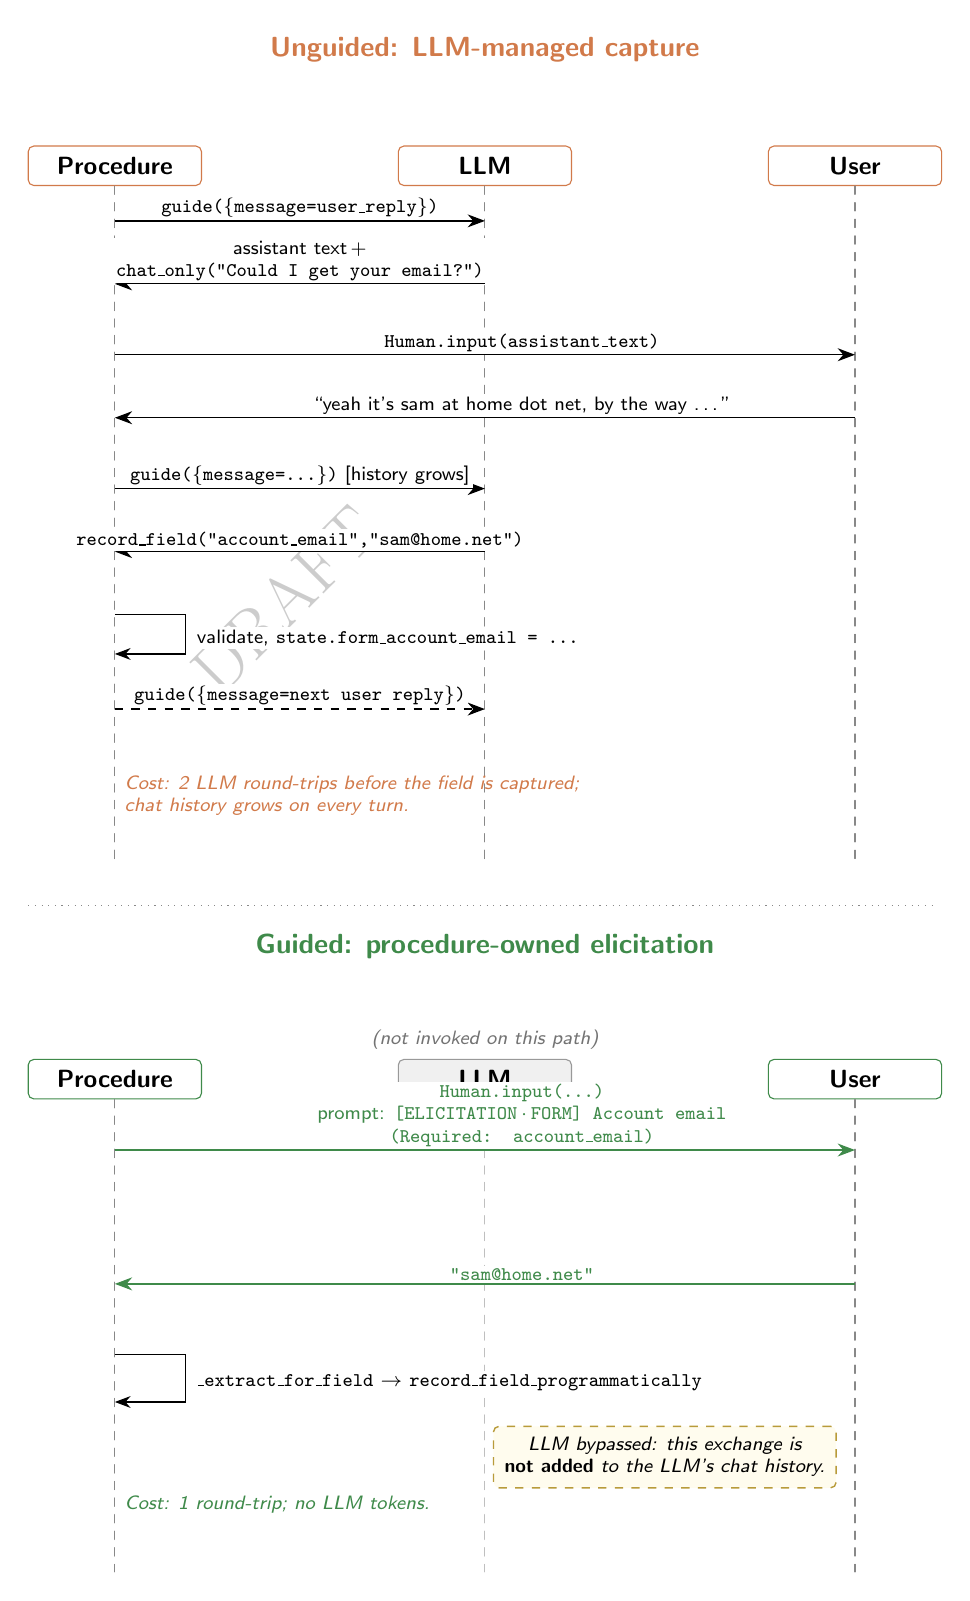
\begin{tikzpicture}[x=1cm,y=1cm,>=Stealth]

% ---------------- UNGUIDED PANEL ----------------
\begin{scope}[shift={(0,0)}]
  \node[panelTitleU, anchor=south] at (5.3,1.2) {Unguided: LLM-managed capture};

  \node[actor, draw=ungOrange] (uProc) at (0.6,0)   {Procedure};
  \node[actor, draw=ungOrange] (uLLM)  at (5.3,0)   {LLM};
  \node[actor, draw=ungOrange] (uUser) at (10.0,0)  {User};

  \draw[lifeline] (uProc.south) -- ++(0,-8.6);
  \draw[lifeline] (uLLM.south)  -- ++(0,-8.6);
  \draw[lifeline] (uUser.south) -- ++(0,-8.6);

  % t1: Procedure -> LLM (current turn)
  \draw[msg] (0.6,-0.7) -- (5.3,-0.7)
    node[msglbl, midway, above] {\texttt{guide(\{message=user\_reply\})}};
  % t2: LLM -> Procedure (assistant text + tool choice)
  \draw[msg] (5.3,-1.5) -- (0.6,-1.5)
    node[msglbl, midway, above, align=center]
        {assistant text\,+\\\texttt{chat\_only("Could I get your email?")}};
  % t3: Procedure -> User
  \draw[msg] (0.6,-2.4) -- (10.0,-2.4)
    node[msglbl, pos=0.55, above] {\texttt{Human.input(assistant\_text)}};
  % t4: User -> Procedure (free-form)
  \draw[msg] (10.0,-3.2) -- (0.6,-3.2)
    node[msglbl, pos=0.45, above] {``yeah it's sam at home dot net, by the way \dots''};
  % t5: Procedure -> LLM (next turn, with growing history)
  \draw[msg] (0.6,-4.1) -- (5.3,-4.1)
    node[msglbl, midway, above] {\texttt{guide(\{message=\dots\})} [history grows]};
  % t6: LLM -> Procedure (tool call)
  \draw[msg] (5.3,-4.9) -- (0.6,-4.9)
    node[msglbl, midway, above] {\texttt{record\_field("account\_email","sam@home.net")}};
  % t7: Procedure validates (self-loop)
  \draw[selfmsg] (0.6,-5.7) -- ++(0.9,0) -- ++(0,-0.5) -- ++(-0.9,0);
  \node[msglbl, anchor=west, align=left] at (1.6,-6.0)
       {validate, \texttt{state.form\_account\_email = \dots}};
  % t8: Procedure -> LLM next turn ack (optional)
  \draw[msg, dashed] (0.6,-6.9) -- (5.3,-6.9)
    node[msglbl, midway, above] {\texttt{guide(\{message=next user reply\})}};
  \node[anchor=west, font=\sffamily\scriptsize\itshape, color=ungOrange,
        align=left] at (0.6,-8.0)
       {Cost: 2 LLM round-trips before the field is captured;\\
        chat history grows on every turn.};
\end{scope}

% Separator
\draw[rulegray, dotted] (-0.5,-9.4) -- (11.0,-9.4);

% ---------------- GUIDED PANEL ----------------
\begin{scope}[shift={(0,-11.6)}]
  \node[panelTitleG, anchor=south] at (5.3,1.4) {Guided: procedure-owned elicitation};

  \node[actor, draw=guGreen] (gProc) at (0.6,0)   {Procedure};
  \node[actor, draw=black!40, fill=black!6] (gLLM) at (5.3,0)  {LLM};
  \node[font=\sffamily\scriptsize\itshape, color=black!55, align=center]
       at (5.3,0.5) {(not invoked on this path)};
  \node[actor, draw=guGreen] (gUser) at (10.0,0)  {User};

  \draw[lifeline] (gProc.south) -- ++(0,-6.0);
  \draw[lifeline, color=black!25] (gLLM.south)  -- ++(0,-6.0);
  \draw[lifeline] (gUser.south) -- ++(0,-6.0);

  % t1: Procedure -> User direct elicitation
  \draw[msg, color=guGreen, line width=0.6pt] (0.6,-0.9) -- (10.0,-0.9)
    node[msglbl, pos=0.55, above, align=center]
       {\texttt{Human.input(\dots)}\\
        prompt: \texttt{[ELICITATION\,$\cdot$\,FORM] Account email}\\
        \texttt{(Required: account\_email)}};
  % t2: User -> Procedure (single response)
  \draw[msg, color=guGreen, line width=0.6pt] (10.0,-2.6) -- (0.6,-2.6)
    node[msglbl, pos=0.45, above] {\texttt{"sam@home.net"}};
  % t3: Procedure self: extract + validate + store
  \draw[selfmsg] (0.6,-3.5) -- ++(0.9,0) -- ++(0,-0.6) -- ++(-0.9,0);
  \node[msglbl, anchor=west, align=left] at (1.6,-3.85)
       {\texttt{\_extract\_for\_field} $\to$ \texttt{record\_field\_programmatically}};

  % Annotation: LLM bypassed
  \node[note, anchor=north west, align=center] at (5.4,-4.4)
       {LLM bypassed: this exchange is\\
        \textbf{not added} to the LLM's chat history.};

  \node[anchor=west, font=\sffamily\scriptsize\itshape, color=guGreen,
        align=left] at (0.6,-5.4)
       {Cost: 1 round-trip; no LLM tokens.};
\end{scope}

\end{tikzpicture}
\caption{Per-step timing for capturing one structured field (\texttt{account\_email}).
Top: under LLM-managed capture, the procedure must round-trip through the LLM to
ask the question, again to interpret the user's reply, and again to emit the
\texttt{record\_field} tool call; chat history grows monotonically. Bottom: under
procedure-owned elicitation, the procedure speaks directly to the user via
\texttt{Human.input} (here using the literal \texttt{[ELICITATION\,$\cdot$\,FORM]}
header used by the implementation), parses and validates the response, and never
invokes the LLM for this exchange. Both panels are drawn from the actual Lua
procedures.}
\label{fig:sequence}
\end{figure}

\subsection{What the LLM actually sees per request}

The second comparison is at the level of one LLM request, mid-conversation. Figure~\ref{fig:context} shows the input context---static system prompt plus accumulated chat history---that each arm sends. Two implementation details, both faithful to the code, appear here for the first time and matter for how the rest of the paper should be read. First, the agent runtime sets a single static \texttt{system}-role message at agent-construction time; both arms use this slot, but the guided arm's text is much shorter because most procedural detail is enforced procedurally rather than instructed. Second, the guided arm communicates per-step instructions to its own LLM by appending them to user-role turns, prefixed with the literal token \texttt{SYSTEM:}. The procedure's own elicitation exchanges with the user are not present in the LLM context at all; we depict them as a dashed out-of-band callout.

\begin{figure}[htbp]
\centering
\resizebox{\linewidth}{!}{%
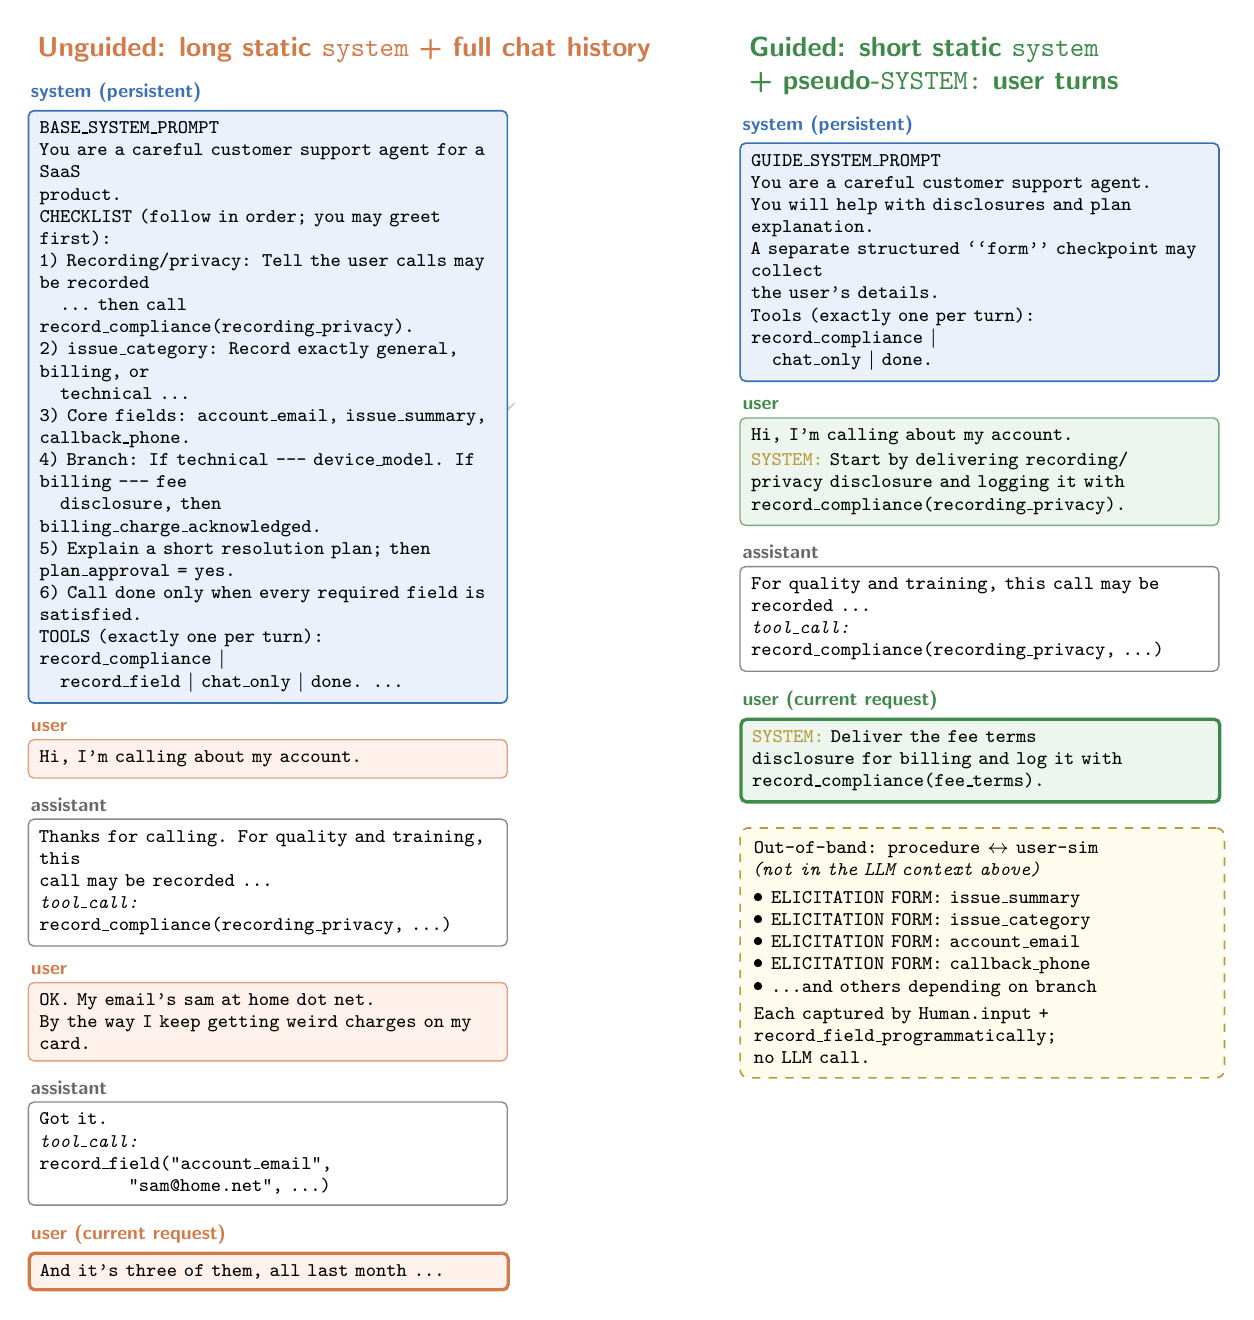
\begin{tikzpicture}[
    font=\sffamily,
    node distance=2mm and 6mm,
    msgRow/.style={inner sep=0pt},
]

% =======================  UNGUIDED column  =======================
\node[panelTitleU, align=left] (uTitle)
     {Unguided: long static \texttt{system} + full chat history};

\node[roleTag, color=taskBlue, below=1mm of uTitle.south west, anchor=north west]
     (uTagS) {system (persistent)};
\node[sysCard, below=0.5mm of uTagS.south west, anchor=north west] (uS)
     {\textbf{BASE\_SYSTEM\_PROMPT}\\
      You are a careful customer support agent for a SaaS\\
      product.\\
      CHECKLIST (follow in order; you may greet first):\\
      1) Recording/privacy: Tell the user calls may be recorded\\
      \quad\dots\ then call \texttt{record\_compliance(recording\_privacy)}.\\
      2) issue\_category: Record exactly general, billing, or\\
      \quad technical \dots\\
      3) Core fields: account\_email, issue\_summary, callback\_phone.\\
      4) Branch: If technical --- device\_model. If billing --- fee\\
      \quad disclosure, then billing\_charge\_acknowledged.\\
      5) Explain a short resolution plan; then plan\_approval = yes.\\
      6) Call done only when every required field is satisfied.\\
      TOOLS (exactly one per turn): record\_compliance $|$\\
      \quad record\_field $|$ chat\_only $|$ done. \dots};

\node[roleTag, color=ungOrange, below=2mm of uS.south west, anchor=north west]
     (uTagU1) {user};
\node[userCard, below=0.5mm of uTagU1.south west, anchor=north west] (uU1)
     {Hi, I'm calling about my account.};

\node[roleTag, color=black!60, below=2mm of uU1.south west, anchor=north west]
     (uTagA1) {assistant};
\node[asstCard, below=0.5mm of uTagA1.south west, anchor=north west] (uA1)
     {Thanks for calling. For quality and training, this\\
      call may be recorded \dots\\
      \textit{tool\_call:}\\
      \texttt{record\_compliance(recording\_privacy, \dots)}};

\node[roleTag, color=ungOrange, below=2mm of uA1.south west, anchor=north west]
     (uTagU2) {user};
\node[userCard, below=0.5mm of uTagU2.south west, anchor=north west] (uU2)
     {OK. My email's sam at home dot net.\\
      By the way I keep getting weird charges on my card.};

\node[roleTag, color=black!60, below=2mm of uU2.south west, anchor=north west]
     (uTagA2) {assistant};
\node[asstCard, below=0.5mm of uTagA2.south west, anchor=north west] (uA2)
     {Got it.\\
      \textit{tool\_call:}\\
      \texttt{record\_field("account\_email",}\\
      \texttt{\quad\quad\quad\quad\,\,"sam@home.net", \dots)}};

\node[roleTag, color=ungOrange, below=2mm of uA2.south west, anchor=north west]
     (uTagU3) {user (current request)};
\node[userCard, draw=ungOrange, line width=1.2pt,
      below=0.5mm of uTagU3.south west, anchor=north west] (uU3)
     {And it's three of them, all last month \dots};

% =======================  GUIDED column  =======================
\node[panelTitleG, align=left, right=10mm of uTitle.north east, anchor=north west]
     (gTitle)
     {Guided: short static \texttt{system}\\
      + pseudo-\texttt{SYSTEM:} user turns};

\node[roleTag, color=taskBlue, below=1mm of gTitle.south west, anchor=north west]
     (gTagS) {system (persistent)};
\node[sysCardSmall, below=0.5mm of gTagS.south west, anchor=north west] (gS)
     {\textbf{GUIDE\_SYSTEM\_PROMPT}\\
      You are a careful customer support agent.\\
      You will help with disclosures and plan explanation.\\
      A separate structured ``form'' checkpoint may collect\\
      the user's details.\\
      Tools (exactly one per turn): record\_compliance $|$\\
      \quad chat\_only $|$ done.};

\node[roleTag, color=guGreen, below=2mm of gS.south west, anchor=north west]
     (gTagU1) {user};
\node[userCardG, below=0.5mm of gTagU1.south west, anchor=north west] (gU1)
     {Hi, I'm calling about my account.\\[1pt]
      \textcolor{oobAmber}{\textbf{SYSTEM:}} Start by delivering recording/\\
      privacy disclosure and logging it with\\
      \texttt{record\_compliance(recording\_privacy)}.};

\node[roleTag, color=black!60, below=2mm of gU1.south west, anchor=north west]
     (gTagA1) {assistant};
\node[asstCard, below=0.5mm of gTagA1.south west, anchor=north west] (gA1)
     {For quality and training, this call may be\\
      recorded \dots\\
      \textit{tool\_call:}\\
      \texttt{record\_compliance(recording\_privacy, \dots)}};

\node[roleTag, color=guGreen, below=2mm of gA1.south west, anchor=north west]
     (gTagU2) {user (current request)};
\node[userCardG, draw=guGreen, line width=1.2pt,
      below=0.5mm of gTagU2.south west, anchor=north west] (gU2)
     {\textcolor{oobAmber}{\textbf{SYSTEM:}} Deliver the fee terms\\
      disclosure for billing and log it with\\
      \texttt{record\_compliance(fee\_terms)}.};

% Out-of-band callout: elicitations the LLM never saw.
\node[oobCallout, below=3mm of gU2.south west, anchor=north west] (gOOB)
     {\textbf{Out-of-band: procedure $\leftrightarrow$ user-sim}\\
      \textit{(not in the LLM context above)}\\[2pt]
      \textbullet\ ELICITATION FORM: issue\_summary\\
      \textbullet\ ELICITATION FORM: issue\_category\\
      \textbullet\ ELICITATION FORM: account\_email\\
      \textbullet\ ELICITATION FORM: callback\_phone\\
      \textbullet\ \dots and others depending on branch\\[2pt]
      Each captured by \texttt{Human.input} +\\
      \texttt{record\_field\_programmatically};\\
      no LLM call.};

\end{tikzpicture}%
}
\caption{The LLM's input context for one mid-conversation request, under each
arm. Both arms send a single static \texttt{system} message at the top of every
request---there is no role-swapping ``ephemeral system message'' on the wire.
What differs is (a) the size of the static prompt, (b) the contents of the
\texttt{user} turns, and (c) what is \emph{absent}. In the guided arm, several
procedure-issued instructions are injected as user-role messages prefixed with
the literal token \texttt{SYSTEM:} (highlighted), and most structured-data
capture happens in out-of-band \texttt{Human.input} exchanges (the dashed
callout) that never enter the LLM's chat history. We name this
``pseudo-\texttt{SYSTEM:}'' injection mechanism explicitly in
Section~\ref{sec:limits}.}
\label{fig:context}
\end{figure}

\subsection{Architecture summary}

Figure~\ref{fig:policy} steps back to the architecture level. Both arms share the same task substrate---validators, simulator, and model---and differ only in which component initiates structured capture. The remainder of the paper makes this contrast concrete on a constrained support-intake benchmark.

\begin{figure}[htbp]
  \centering
  \includegraphics[width=0.95\linewidth]{control_policy.pdf}
  \caption{The same diagram at the architecture level. Both arms share
  task, validators, simulator, and model. The unguided arm routes capture
  through inline LLM tool calls; the guided arm routes capture through
  procedure-owned \texttt{elicitation\_form} checkpoints. The remainder of
  the paper makes this comparison concrete on a constrained support-intake
  benchmark.}
  \label{fig:policy}
\end{figure}

% =============================================================================
\section{Benchmark}
\label{sec:benchmark}

\subsection{Task and constraints}

The benchmark models a phone-style customer support intake. A run is a multi-turn conversation between the agent and a simulated user. Successful intake requires, in order or with documented enforcement:

\begin{enumerate}[noitemsep,leftmargin=2em]
    \item recording/privacy disclosure (compliance) before any account identifier;
    \item issue category classification, restricted to \texttt{general}, \texttt{billing}, or \texttt{technical};
    \item core fields: \texttt{account\_email}, \texttt{issue\_summary}, \texttt{callback\_phone};
    \item branch-specific fields (\texttt{device\_model} for technical; fee disclosure plus \texttt{billing\_charge\_acknowledged} for billing);
    \item a brief plan explanation followed by an explicit \texttt{plan\_approval} acknowledgment;
    \item a final \texttt{done} call.
\end{enumerate}

These rules are enforced by Lua validators and procedure-side guards. Field-level constraints include format checks (phone \texttt{XXX-XXX-XXXX}, plausible email), minimum lengths, and exact-string acknowledgments (\texttt{yes}). The same validator set is used in both arms.

\subsection{Personas}

Three personas isolate different stress patterns (Table~\ref{tab:personas}). Each persona has a private ground-truth dictionary covering all branch-specific requirements; ground truth is held constant across runs.

\begin{table}[htbp]
  \centering
  \small
  \caption{Personas and the structured fields each one ultimately needs to disclose.}
  \label{tab:personas}
  \begin{tabular}{lll}
    \toprule
    Persona & Branch & Distinctive challenge \\
    \midrule
    \texttt{support\_rambler}   & general    & buries answers in long stories \\
    \texttt{support\_billing}   & billing    & extra fee disclosure + ack + approval \\
    \texttt{support\_technical} & technical  & extra device-model branch field \\
    \bottomrule
  \end{tabular}
\end{table}

\section{Control policies, concretely}
\label{sec:policies}

Section~\ref{sec:capture} introduced the conceptual contrast and Figures~\ref{fig:sequence}--\ref{fig:policy} illustrate the mechanism. This section pins down the implementation surface so the comparison is reproducible.

\paragraph{Unguided.}
The unguided arm exposes the tool surface \texttt{record\_field}, \texttt{record\_compliance}, \texttt{chat\_only}, \texttt{done} to the LLM, with \texttt{tool\_choice = required} so every turn must emit exactly one tool call. The procedure runs validators inside each tool handler but does not initiate capture; it advances state in response to whatever the model emits.

\paragraph{Guided.}
The guided arm exposes a strictly smaller surface: \texttt{record\_compliance}, \texttt{chat\_only}, \texttt{done}. \texttt{record\_field} is intentionally absent; field capture is structurally unavailable to the model. Instead, the procedure issues \texttt{elicitation\_form} checkpoints (Figure~\ref{fig:sequence}, bottom panel) that read directly from the user via \texttt{Human.input} and store validated values via \texttt{record\_field\_programmatically}.

\paragraph{What is held constant.}
Both arms use the same persona-grounded simulator, the same model (\texttt{gpt-5.4-mini}) for both the agent and the simulator, the same maximum-turn budget ($58$ user rounds per run, plus the underlying procedure-internal turn cap), the same set of validators, and the same outcome classification.

\section{Simulated user and protocol}
\label{sec:protocol}

\subsection{Simulator}

We replace human input with \texttt{LLMHITLHandler}, a fast model role-playing the persona using the persona's private ground-truth dictionary. For ordinary conversational turns, the simulator generates user replies in character.

\paragraph{Behavior at elicitation prompts.}
At elicitation-form prompts (recognized by the \texttt{[ELICITATION\,$\cdot$\,FORM]} sentinel header used in Figure~\ref{fig:sequence}), the simulator returns the requested ground-truth field value directly rather than improvising a paraphrase. This mirrors the design intent of MCP-style elicitation: a real client renders a structured request to the user and submits the user's structured response, not a free-text paraphrase. We discuss the implications of this choice in Section~\ref{sec:limits}.

\subsection{Outcome classification}

Each rollout terminates with one of four outcomes (Figure~\ref{fig:outcomes}):
\begin{itemize}[noitemsep,leftmargin=2em]
    \item \textbf{infra\_error}: execute/API failure;
    \item \textbf{incomplete}: ran without infra failure but never legitimately reached \texttt{done};
    \item \textbf{completed\_strict\_fail}: reached \texttt{done} but at least one ground-truth field is wrong, missing, or malformed;
    \item \textbf{strict\_ok}: reached \texttt{done} with every ground-truth field passing its per-field check (see below).
\end{itemize}

\paragraph{Per-field policy.}
Branch-critical and identifier fields (\texttt{account\_email}, \texttt{callback\_phone}, \texttt{issue\_category}, \texttt{device\_model}) require exact match against ground truth after lowercasing and trimming, and boolean acknowledgments (\texttt{billing\_charge\_acknowledged}, \texttt{plan\_approval}) require an exact boolean match. \texttt{issue\_summary} is treated as a free-text field and is required only to be non-empty with at least five characters; we do not impose semantic equivalence on it because no downstream system in the modeled workflow consumes the summary as a structured key.

\begin{figure}[htbp]
  \centering
  \includegraphics[width=0.95\linewidth]{outcomes.pdf}
  \caption{Outcome classification pipeline used in this study. Strict success counts only \texttt{strict\_ok}; completion counts both \texttt{strict\_ok} and \texttt{completed\_strict\_fail}; infra failure isolates execute/API errors so they cannot be charged to either policy.}
  \label{fig:outcomes}
\end{figure}

\subsection{Metrics}

We report:
\begin{itemize}[noitemsep,leftmargin=2em]
    \item \textbf{Strict success (excluding infra)}: \texttt{strict\_ok} runs divided by non-infra runs;
    \item \textbf{Completion}: \texttt{strict\_ok} $+$ \texttt{completed\_strict\_fail}, divided by all runs;
    \item \textbf{Infra failure rate}: infra runs divided by all runs.
\end{itemize}
Confidence intervals are Wilson 95\% intervals for each binomial proportion; deltas are reported in percentage points.

\subsection{Study configuration}

The canonical run reported below uses tag \texttt{eval100\_elic\_paper1} with \texttt{RELIABILITY\_RUNS=100} per persona per arm, \texttt{RELIABILITY\_CONCURRENCY=10}, paired user simulation (\texttt{RELIABILITY\_PAIR\_USER\_SIM=1}), and one-shot infra retry (\texttt{RELIABILITY\_RETRY\_INFRA=1}). Total executions: $2 \times 3 \times 100 = 600$.

\section{Results}
\label{sec:results}

\subsection{Headline outcomes}

Table~\ref{tab:strict} reports strict success excluding infra failures; Table~\ref{tab:completion} reports completion; infra failures were $0\%$ in every cell, so strict and strict-excluding-infra rates coincide. The guided arm produces no failures of any kind in this study. The unguided arm completes a minority of runs in every persona, with billing the hardest path.

\begin{table}[htbp]
  \centering
  \caption{Strict success (excluding infra). $n=100$ per persona per arm; Wilson 95\% intervals.}
  \label{tab:strict}
  \begin{tabular}{lccc}
    \toprule
    Persona & Unguided & Guided & $\Delta$ (G$-$U) \\
    \midrule
    \texttt{support\_rambler}   & $54\%$ $[44.3, 63.4]$ & $100\%$ $[96.3, 100.0]$ & $+46$ pp \\
    \texttt{support\_billing}   & $41\%$ $[31.9, 50.8]$ & $100\%$ $[96.3, 100.0]$ & $+59$ pp \\
    \texttt{support\_technical} & $52\%$ $[42.3, 61.5]$ & $100\%$ $[96.3, 100.0]$ & $+48$ pp \\
    \midrule
    Equal-weighted mean         & $49.0\%$              & $100.0\%$               & $+51$ pp \\
    \bottomrule
  \end{tabular}
\end{table}

\begin{table}[htbp]
  \centering
  \caption{Completion. $n=100$ per persona per arm; Wilson 95\% intervals.}
  \label{tab:completion}
  \begin{tabular}{lccc}
    \toprule
    Persona & Unguided & Guided & $\Delta$ (G$-$U) \\
    \midrule
    \texttt{support\_rambler}   & $61\%$ $[51.2, 70.0]$ & $100\%$ $[96.3, 100.0]$ & $+39$ pp \\
    \texttt{support\_billing}   & $44\%$ $[34.7, 53.8]$ & $100\%$ $[96.3, 100.0]$ & $+56$ pp \\
    \texttt{support\_technical} & $56\%$ $[46.2, 65.3]$ & $100\%$ $[96.3, 100.0]$ & $+44$ pp \\
    \midrule
    Equal-weighted mean         & $53.7\%$              & $100.0\%$               & $+46$ pp \\
    \bottomrule
  \end{tabular}
\end{table}

\subsection{Outcome decomposition}

The outcome decomposition (Table~\ref{tab:outcomes}) tells a sharper story than the rates alone: most unguided failures are not \emph{wrong} answers, they are \emph{absent} ones. Across personas, $46.3\%$ of unguided runs ($139/300$) ended as \texttt{incomplete}, while only $4.7\%$ ($14/300$) were \texttt{completed\_strict\_fail}. The unguided arm, in other words, is generally honest about its structured outputs when it manages to finish; its dominant problem is finishing.

\begin{table}[htbp]
  \centering
  \small
  \caption{Outcome decomposition for the unguided arm ($n=100$ per persona). Guided cells are $100\%$ \texttt{strict\_ok} and are omitted.}
  \label{tab:outcomes}
  \begin{tabular}{lrrr}
    \toprule
    Persona & \texttt{strict\_ok} & \texttt{incomplete} & \texttt{completed\_strict\_fail} \\
    \midrule
    \texttt{support\_rambler}   & $54$ & $39$ & $7$ \\
    \texttt{support\_billing}   & $41$ & $56$ & $3$ \\
    \texttt{support\_technical} & $52$ & $44$ & $4$ \\
    \midrule
    Total                       & $147$ & $139$ & $14$ \\
    \bottomrule
  \end{tabular}
\end{table}

\subsection{Failure fields and turns-to-resolution}

Among the $14$ unguided runs that finished but failed strictness, the dominant culprit is \texttt{issue\_category} ($12$ mismatches), followed by \texttt{device\_model} ($4$); other fields appear at most twice (Table~\ref{tab:failures}). These are exactly the choice points where one wrong commitment cascades through later branch-specific requirements.

\begin{table}[htbp]
  \centering
  \caption{Top mismatched fields among unguided \texttt{completed\_strict\_fail} runs, summed over personas ($n=14$).}
  \label{tab:failures}
  \begin{tabular}{lr}
    \toprule
    Field & Mismatches \\
    \midrule
    \texttt{issue\_category}              & $12$ \\
    \texttt{device\_model}                & $4$  \\
    \texttt{callback\_phone}              & $2$  \\
    \texttt{billing\_charge\_acknowledged}& $1$  \\
    \texttt{compliance\_fee\_done}        & $1$  \\
    \bottomrule
  \end{tabular}
\end{table}

The turn distribution makes the cost of unguided failure concrete. Successful unguided rollouts averaged $20.3$ user turns ($\min 7$, $\max 94$). Failed unguided rollouts averaged $95.6$ user turns---close to the per-run cap of $110$ underlying turns---across $153$ failed runs (Table~\ref{tab:turns}). Guided rollouts terminated in $2$--$3$ turns (mean $2.3$); we discuss this efficiency number explicitly in Section~\ref{sec:limits}, since most of it reflects checkpoint behavior at the simulator side rather than a clean ``the model is just faster'' story.

\begin{table}[htbp]
  \centering
  \caption{User-turn statistics by arm and outcome class. Failed unguided rollouts approach the procedure cap, indicating exhaustive recovery attempts rather than quick give-ups.}
  \label{tab:turns}
  \begin{tabular}{llrrrr}
    \toprule
    Arm & Outcome class & $n$ & mean & min & max \\
    \midrule
    Unguided & \texttt{strict\_ok}                & $147$ & $20.3$ & $7$  & $94$  \\
    Unguided & not \texttt{strict\_ok}            & $153$ & $95.6$ & $11$ & $111$ \\
    Guided   & \texttt{strict\_ok}                & $300$ & $2.3$  & $2$  & $3$   \\
    \bottomrule
  \end{tabular}
\end{table}

\section{Discussion}
\label{sec:discussion}

\subsection{What kind of failure does checkpoint ownership remove?}

The decomposition in Table~\ref{tab:outcomes} suggests that the unguided baseline does not primarily fail by lying about structured state; it fails by getting stuck. Failed unguided runs concentrate near the per-run turn cap (Table~\ref{tab:turns}), which is consistent with the model repeatedly trying---and failing---to recover ordering or branch invariants on its own. Once the procedure owns the timing of branch-critical capture (guided arm), those recovery loops disappear: the procedure asks for the precise field it needs, validates the answer, and either advances or asks again.

This is the intended mechanism of the intervention: the intervention does not make the LLM ``smarter'' about which field to ask for; it removes the meta-level task of choosing when to ask. The completed-strict-fail count for unguided is small ($14$ across $300$ runs), and the dominant culprit is \texttt{issue\_category}, the single decision that controls every downstream branch-specific requirement. A wrong commitment there leaves the model trying to satisfy the wrong checklist for the rest of the run, which both lowers strict success and inflates turns-to-resolution.

\subsection{Why is billing the hardest persona for the baseline?}

Billing exhibits both the lowest unguided completion ($44\%$) and the largest strict-success gap ($+59$ percentage points, the largest of the three personas). Billing is also the persona with the most ordering-sensitive obligations: a fee disclosure must occur before \texttt{billing\_charge\_acknowledged}, and \texttt{plan\_approval} must follow a plan explanation. The pattern is consistent with the mechanism described above: more required orderings mean more places where an LLM-driven capture policy can stall or commit to the wrong branch.

\subsection{What the gain does \emph{not} say}

The 100-vs-49\% headline is a claim about a control architecture, not about the LLM's competence; under matched conditions, moving the timing decision out of the conversational policy is sufficient to close essentially all of the observed reliability gap on this benchmark. The guided arm's $2.3$-turn average is shaped by the simulator's idealized response at elicitation prompts and should not be read as a production latency claim.

\section{Threats to validity and limitations}
\label{sec:limits}

\paragraph{Pseudo-\texttt{SYSTEM:} injection in the guided arm.}
Figure~\ref{fig:context} shows that the guided procedure's mid-run instructions to its own LLM (e.g.\ ``Deliver the fee terms disclosure for billing'') are not delivered as a separate \texttt{system}-role message; they are appended to a \texttt{user}-role turn whose content begins with the literal token \texttt{SYSTEM:}. We adopted this mechanism because the underlying agent runtime sets one persistent system prompt at agent-construction time and does not support per-turn role-swapping. A more idealized implementation would inject these as true ephemeral system messages. We do not have evidence that this mechanism alone explains the gap, but it is part of how the guided arm is implemented and we want to name it explicitly rather than hide it.

\paragraph{Simulator--checkpoint interaction (internal/construct validity).}
At elicitation prompts, the simulator responds with the requested ground-truth field directly. This mirrors the design intent of MCP-style elicitation---a client renders a structured request to a real user who then submits a structured response---but it also means that, in our harness, every guided checkpoint is answered with a value that will pass validation. Some portion of the guided arm's reliability gain therefore reflects the simulator behavior that is paired with the intervention, not the intervention alone. We adopt this design because it is the natural simulator analog for the architecture we are studying, but we want to flag, rather than hide, that a noisier client-side response policy would likely move the guided rates downward.

\paragraph{Single task, single model.}
The benchmark is one constrained-intake workflow with one branching structure, evaluated with one model family (\texttt{gpt-5.4-mini}) for both the agent and the simulator. We do not claim the percentage-point magnitudes generalize; we claim the qualitative direction is consistent with the mechanism we describe.

\paragraph{Construct validity of strict success.}
Strict success applies exact-after-normalization match to fields where the workflow itself requires exactness (identifiers, branch choices, boolean acknowledgments) and a non-empty / minimum-length check to \texttt{issue\_summary}, where a real downstream system would accept any reasonable description of the problem. This split reflects the surrounding workflow's own definition of correctness, but readers with stricter or more semantic metrics in mind should weight that asymmetry when interpreting the rates: a fully semantic metric would weaken the comparison on \texttt{issue\_summary} only, while a fully strict metric across all fields would tighten it.

\paragraph{Turn-budget interaction.}
Failed unguided runs approach the per-run turn cap, which means the unguided baseline is benefiting from being allowed to retry but is also losing runs to the cap. Different caps would shift the absolute completion number but not the comparison's direction.

\paragraph{Efficiency interpretation.}
The very low guided turn count ($\approx2.3$) should not be reported in isolation as a UX result. With a real client, those turns expand into the user's actual answering time per checkpoint. Treat the number as an indicator that the guided arm avoids exploratory loops, not as an end-to-end latency claim.

\section{Conclusion}

In a constrained support-intake benchmark with three personas and $600$ rollouts, moving authoritative structured capture out of an LLM-managed conversation and into procedure-owned elicitation checkpoints raises strict success from $49.0\%$ to $100\%$ and completion from $53.7\%$ to $100\%$, with $0\%$ infrastructure failures in either arm. A failure-mode decomposition shows that the gain is driven primarily by eliminating \emph{incomplete} runs in which the unguided baseline exhausts its turn budget trying to recover from ordering or branching mistakes; the magnitude of the gap is shaped, but not reversed, by the simulator's idealized response at checkpoints. We expect the same control-architecture lever to apply to other constrained-intake patterns---regulated triage, claims intake, structured onboarding, compliance workflows, and service-desk routing---wherever a workflow's definition of \emph{done} requires exact structured fields collected in a specified order. The result supports a scoped recommendation: when an agentic workflow has hard procedural constraints and exact structured output requirements, ownership of capture timing is a strong reliability lever, and is largely orthogonal to the choice of model.

\end{document}
